\documentclass[11pt,a4paper]{article}
\usepackage[latin1]{inputenc}
\usepackage{amsmath}
\usepackage{amsfonts}
\usepackage{amssymb}
\usepackage{graphicx}
\usepackage{titling}
\usepackage{color}
\usepackage[final]{pdfpages}
\newcommand{\abbr}[1]{\textsc{\texttt{#1}}}
\newcommand{\abbrlc}[2]{\textsc{\texttt{#1}}\texttt{#2}}
\author{Michael C. Kunkel}
\date{}
\title{Comment to Reviewers on "Measurement of Cross-Sections of exclusive $\pi^{0}$ Photo-production on Hydrogen from 1.1 GeV - 5.45 GeV using $\lowercase{e}^{+}\lowercase{e}^{-}\gamma$ decay from the CLAS/g12 Data"}
\begin{document}
\maketitle
\section{First remarks}
Author hopes that reply to committee's review is not taken in an offending manner. All replies, after section ``Impression of committee'', are hoped to be taken as a scientific discussion.
\section{Impression of committee}
There is an overall sentiment that the committee, whom has two g12 members, did not communicate effectively to the third member the goal of the g12 analysis procedure. Some of the comments given were redundant to each other. Some questions were already known by the two g12 members, as this note was presented to them within 2 weeks of submission. Author feels like the overall goal that the g12 analysis note procedure was trying to achieve was not met by this committee. Author's impression has already been brought up in g12 meeting, and received a general agreement with one committee member.
\section*{Preamble}
\textcolor{red}{This final state is the sum of two subprocesses, the $\pi^0$ meson decay through the three-body Dalitz decay...}
\textcolor{blue}{It should be noted that the ``Dalitz decay'' is not a three-body decay. It is  two-body decay of $\pi^0$ where one(or both) of the photons is off-shell. Then the subsequent off-shell photon decays into a $e^+e-$ pair.}
\section*{General Concerns}
\begin{enumerate}
\item
\textcolor{red}{Is it justified to quote a global uncertainty for the sector dependence and the track dependent particle efficiencies if they were actually extracted on a bin-by-bin basis? Why not quote the bin- by-bin uncertainty rather than a global one?}
\textcolor{blue}{Yes, when the number quoted is the upper limit. A bin-by-bin is not possible with the binning used in the analysis. Since the sector systematic was energy dependent, adding a third, very fine binned, dimension would not have been possible. }
\item
\textcolor{red}{Some of the g12/g1c comparisons that are on a log scale might be misleading. Is there a pull distribution for g12/g1c}
\textcolor{blue}{G12 analysis note Fig. 152}
\item
\textcolor{red}{fiducial cuts. These are not mentioned explicitly within the procedure of the analysis. We understand that those are standard approved cuts, so no need to expand a lot about these, but as you describe the line of the analysis, explicitly mention at the appropriate stage that fiducial cuts were applied (as was done with the reference to target density for example in chapter 3).}
\textcolor{blue}{Added a section which is before description of track efficiency. It reads ``Fiducial cuts for g12 were derived and appropriately described in g12note. For this analysis, fiducial cuts were performed prior the the application of the track efficiency described in Sec.6 }
\item
\begin{enumerate}
\item
\textcolor{red}{it seems that the normalization correction accounts for two effects: (a) differences in the real and simulated detector resolutions (any geometric mismatch in detector position and orientation would be convoluted mostly with the resolutions ?}
\textcolor{blue}{Yes, however g12 calibration index had a DC bank that took into account the geometric rotations of the DC, therefore this effect would be second order compared to the DC resolution comparison}
\item 
\textcolor{red}{(b) differences in various detector elements finite efficiencies. The former would be especially pronounced at the edges of the detector (geometric edges or minimum momentum edges). The latter would be edge unrelated. In order to be able to judge how well the simulation resolution matches the detector resolution, we would like to see extra figures (in addition to missing mass and momentum and angle distributions which are given throughout the note) from this analysis for differences of momenta and angles (reconstructed - measured) of each of the three particles for both the simulated and the real data.}
\textcolor{blue}{Not feasible, as this data/scripts were lost during the cluster upgrade in which the g12 work disk was affected. The two committee members whom are g12 members know of this situation. See comment 15 in ``More specific comments'', in which this topic is also discussed in terms of DC calibration.}
\end{enumerate}
\item
\textcolor{red}{We would like to see more detail on the method by which the systematic uncertainty (error) of the normalization correction was determined. This is a large correction, which absorbs some acceptance and resolution effects, but is only 0.5\%? That small value may be perfectly valid, but we are surprised since we have not seen any CLAS cross section analysis yet having a smaller acceptance uncertainty better than 5\%. This makes it important to see more details on the method for estimating the 0.5\%. In addition, we would like to see the expression/method used to estimate the statistical uncertainty of 0.01\%}
\textcolor{blue}{In Progress as the original codes are in Germany, I am currently in U.S. Cannot get to the files before December 3, 2016}
\item
\textcolor{red}{Somehow a general but minor concern. It seems to be a loose use of the words ?error? and/ or ?uncertainty? in the note. For example: in Table 50: You quote a "sector systematic uncertainty?, but I guess you mean "acceptance systematic error?. Similar comment for "Particle Efficiency". Make the labels for uncertainties (errors) consistent with the names of the sources you describe earlier in the text.}
\textcolor{blue}{Please refer to comment 29 in ``More specific comments''.}
\end{enumerate}
\section*{More specific comments}
\begin{enumerate}
\item
\textcolor{red}{ page 6 ``missing mass of p(g, p)x off the target proton and the tagged photon.''
should say ``missing mass off the target proton, the tagged photon and the observed proton''.}
\textcolor{blue}{p(g, p)x is generally known as nuclear physics nomenclature.}
\item
\textcolor{red}{page 7 2.2 We do not understand well the cut used to determine e versus pi? We do not understand what you mean to say here. If the track's momentum is consistent with the kinematics of the reaction of interest, then assigning the track the proper e+ or e- track will yield a missing mass consistent with a missing photon (within the missing mass resolution)? Clarify.}
\textcolor{blue}{$\pi^0$ cannot decay to $\pi^+\pi^-$, violates conservation of energy. Therefore when $M_x^2(\gamma p - p) = m_{\pi^0}$, then the skimmed $\pi^+\pi^-$ are misidentified $e^+e^-$}
\item
\textcolor{red}{page 7 sec 2.2: First sentence,"conservation of mass" is misleading (i.e. mass is not conserved). The last sentence in that section is more appropriate.}
\textcolor{blue}{changed}
\item
\textcolor{red}{p.7, table 2: "initial skim selects only events with one in-time beam photon." We could not find later in the note any correction applied to compensate for lost yield due to events with more than ``one in-time photon'' Is it done?}
\textcolor{blue}{The probability that there is a $2^{nd}$ in-time photon detected is 18\% at $E_\gamma$ = 1.1~GeV and $\sim$4\% at $E_\gamma$ = 4.4~GeV and $\sim$2\% at 5.5~GeV. Therefore the chance we choose the incorrect photon is half of these value, i.e. 9\% at $E_\gamma$ = 1.1~GeV and $\sim$2\% at $E_\gamma$ = 4.4~GeV and $\sim$1\% at 5.5~GeV. The track efficiency corrections derived with $p\pi^+\pi^-$ also were affected by this phenomena (i.e. skimmed with only one photon) and corrected this normalization. A study was performed using all in-time photons, see g12 wiki, in which the track efficiency was also calculated with all in-time photons, the difference on the reported results was negligible}
\item
\textcolor{red}{page 8 used. "To satisfy the trigger requirement in the data for photon beam energies
$<$ 3.6 GeV, cuts were placed on the EC and CC hit quantities recorded." Could you expand, it is not clear what that means?}
\textcolor{blue}{The detectors \abbr{CC} and \abbr{EC} generate data when tracks either produce Cherenkov radiation (in the case of the \abbr{CC}). If the number of photo-electron produced in the the Cherenkov gas equals or exceeds the preset gains of the photomultiplier (\abbr{PMT}) then the \abbr{CC} hit bank records a hit status of ``1''. The process is similar for the \abbr{EC} except the physics is a cascade effect of E\&M effects, i.e. ``pair-production'' and ``bremsstrahlung''. The effect of passing the preset gains of the \abbr{PMT} ``trigger'' the event, therefore these quantities must also be used in the analysis where this part of the trigger is applicable This data is stored in the bos-bank and propagated throughout the analysis.}
\item
\textcolor{red}{page 20. 3. Is there a reason to vary the CL cut from 1\% to 10\%, instead, let?s say from 10\% vs 20\%. we are just curious about the reasoning}
\textcolor{blue}{Author does not understand question. Page 20 does not refer to any CL of 1\%, 10\% or 20\%. If the reviewer is referring to page 74, Tab. 13 in the ``Systematics'' section then the decision to use 10\% was that the CL distribution from 1\% to 20\% had the same shape as 1\% to 10\%, therefore author wanted to use the maximum amount of statistics because fo fine binning used.  }
\item
\textcolor{red}{page 25 ``It is shown in Fig. 14a that each cut reduces the background
without significantly reducing the signal.'' That figure seems not to be a good tool to show that. Perhaps we need to quantify? For data sample: Show differences total - signal. For MC data: give numbers : pi0 tot initial. pi0 tot final.}
\textcolor{blue}{Author defers because the figures show clear depression of background, while ``signal'' region is less impacted by imposed cuts.}
\item
\textcolor{red}{ page 28 ``The remainder of the background can be attributed to ...events.'' What background remainder do you mean? The top green distribution in Fig. 14 does not demonstrate what background is remaining. Do you mean for Eg$\geq$3.6 GeV?}
\textcolor{blue}{See Fig. 15 (a)}
\item
\textcolor{red}{page 28 ``The effect of the 75 MeV missing energy cut on the M2
x(p) spectrum can be seen in Fig. 16.'' Figure 16 does not demonstrate the effect of the 75-MeV cut on the data as it does not show distributions before and after the cut. Fig. 16 shows the MM distributions after all the cuts (until that point) have been applied. It also shows the modeling of the signal and the remaining background.}
\textcolor{blue}{Fig 16 (a) does demonstrate the effect when compared to Fig. 14(a). Fig 15 (a) shows the validity of the cut.}
\item
\textcolor{red}{Figure 15. In caption the Mass parenthesis descriptions and the figure axes descriptions should match.}
\textcolor{blue}{Fixed}
\item
\textcolor{red}{page 36. ``This effect was studied as a systematic uncertainty (see Sec 7.3).'' that should be a systematic error and corrected for. Unless the simulation was also applied a Z-vertex cut to in which case the acceptance should take care of this effect and the uncertainty of that becomes part of the acceptance. Unless there is more?}
\textcolor{blue}{See Section 6.5 where there is an statement ``Once the events are processed through \abbr{a1c}, the cuts described in[14], Sec. 6.3, Secs. 2, 2.3.3, are applied as they are to the real data.'' }
\item
\textcolor{red}{ p.40: in section 2.6 the bit 6 pi0 efficiency is studied. We would like more detailed information here. Right now it looks like the total number of entries (what is meant by number of entries - events, hits, else?) for bit 6 is normalized to the total number of pi0 events in bit 6 (at least the top panel of Fig.24 shows the total number of pi0 events and that has been obtained by the analysis of trigger bit 6 only). This looks like a self normalization: bit 6 is normalized to bit 6, is it not then expected that the ratio would be one, independent of efficiency of that trigger bit?}
\textcolor{blue}{For the g12 trigger system, and other \abbr{CLAS} experiments trigger systems, there was no hierarchy in the trigger. This means that no ``bit'' had a higher precedence. Therefore it is always possible that if ``bit 6'' was triggered, that it could have been accompanied by other trigger hits. Trigger information is stored in hexadecimal format, therefore for one reconstructed event the ``bit'' must be ``decoded''. The purpose of section 2.5 of the note, and especially Fig. 25 is to demonstrate the bit efficiency. Using nomenclature such as ``events'', ``hit'' etc. is misleading. The proper word is entries because for one event there can be multiple recordings of different triggers, i.e. entries. Up until section 2.5, there was no assumption on the trigger performance, so statements such as ``at least the top panel of Fig.24 shows the total number of pi0 events and that has been obtained by the analysis of trigger bit 6 only'' are incorrect. What should be understood is that for all events in Fig. 24 (top panle only), the trigger ``bit'' was looked at. In order to show ``efficiency'', the spectrum of trigger entries must be normalized by the number of reported event in Fig. 24 (top panel only). For $\pi^0$ events, trigger ``bit'' 6 was $\sim 100 \%$ efficient, therefore no trigger normalization was needed.}
\item
\textcolor{red}{Were fiducial cuts applied to simulated and real data for the normalization analysis? If so, were exactly the same fiducial cuts applied? In any case put in the note.}
\textcolor{blue}{The purpose of the g12 overall analysis note, and the checklist was to avoid such confusions. Please refer to the checklist.}
\item
\textcolor{red}{Could you explain why the areas of the coils are shown with finite efficiencies if figures 29, 30, 32, 33, and somewhat on figures 35 and 36? The latter two figures seem to show zero efficiency only for two coils (at theta , cos$_{phi}=0$) but not for the diagonal ones - why? Why are figures 29, 30, 32, and 33 not showing any o efficiency for the same two coils as shown by 35 and 36?}
\textcolor{blue}{This topic was already addressed to the member. However for clarity, this study was performed prior to the g12 fiducial cuts being developed. Since fiducial cuts are applied, the values of these bins will never be taken into account.}
\item
\textcolor{red}{Figures 31 and 32 suggest that the normalization corrections are particle dependent. How confident are you (beyond the general argument that both e and pi are minimum ionizing particles) that the pion corrections are applicable to electrons? The direction of my question is leading towards estimating the level of such doubt (i.e. a related uncertainty) in the total systematic uncertainty of the corrections.}
\textcolor{blue}{This is a great question. We debated this in g12 for many months. Although other g12 members know of this argument, the answer was ``We do not know, but when we apply these corrections to $K^+K^-$ topologies, i.e. cascades, the effects are the same. Same results are for $\pi^+\pi^-$, i.e. $\omega\rightarrow\pi^+\pi^-(\pi^0)$ '' Meaning that these corrections work for all particles detected in CLAS, through 1st hand empirical knowledge. We could only conclude that that the track efficiency was some intrinsic property of the detector. After talking with Mac Mestayer, he concludes that there is a overall track dependent efficiency due to the DC calibration. He estimated it at 5\% per track, g12 quotes 6\% per track. }
\item
\textcolor{red}{Figure 38: instead of showing the two estimates on top of each other, can you show the difference between them (the stat. uncertainty of this difference is exactly zero)?}
\textcolor{blue}{Author defers because most points are within errors of each other.}
\item
\textcolor{red}{Could you explain the arguments justifying to apply the g11 overall normalization to the g12 data?}
\textcolor{blue}{We only use this a a cross-check to understand g12 track efficiency. However g11 and g12 only differed by beam energy and target placement. Therefore applying g11 corrections were justified to first order.}
\item
\textcolor{blue}{For the following 19-23, Author notices that the purpose of ``Simulation Verification'' was lost on the committee. This section was only to ``verify'' that the simulation would produce the desired results IFF we apply all physics processes, i.e. cross-section, decay models, etc to a simulation and cross-check the output with data. This section has no relevance on the final simulation, nor final results,  as the final simulation was performed using phasespace.}
\item
\textcolor{red}{Why did you use only e+e- events for verification and not pe+e- events?
- add a last sentence to section 6.1 explaining whether you corrected the cross sections with
any of these inefficiencies.}
\textcolor{blue}{The efficiency of the leptons are not dependent on the efficiency of the proton. This sections describes how we tuned the calibration run index for electron/positron pairs in g12. basically the ``tuning'' was to use all of run 56855 ``run info'' into run 10 but keeping the CC and EC constants from Run 10. No more information can be inferred from this study since the overall final efficiency of the simulation was within 1.1\% of the data.}
\item
\textcolor{red}{This is a clarification comment - I cannot follow the trigger simulation (it is the wording): so 1, 2, and 3 refer to returning the sector number and 4 refers to returning 0 or 1 for that sector? What happens if two sectors simultaneosly satisfy the conditions?}
\textcolor{blue}{If two sectors satisfy the condition, then there were 2 particles that satisfied the individual condition. Each particle has its own trigger simulation boolean.}
\item
\textcolor{red}{You state that the acceptance inefficiency was 1.1\%. (a) Is this value used to correct the final cross sections? (b) after the normalization correction from chapter 5 is applied, do you not expect zero remaining inefficiency of the simulation? This makes me wander how uncertain is this 1.1%?
}
\textcolor{blue}{This value to only demonstrate that the verification of the simulation output, using cross-section models, calculation of g12 photon flux, and VMD $\pi^0$ Daltix decay parameters yielded a result within 1.1\%. None of this information is needed for the results reported in the note.}
\item
\textcolor{red}{Figures 42 - 45 show systematic differences between the simulated and real data - please comment on those: what is the origin? are they accounted for? and if so where?}
\textcolor{blue}{See previous comments on this section}
\item
\textcolor{red}{figure 46 top - show the difference between the two distributions (normalized to the value of the data) with proper uncertainty and comment on the difference - should we worry about it at this point - why or why not.}
\textcolor{blue}{See previous comments on section}
\item
\textcolor{red}{section 6.5 - show the acceptance for the same kinematics as you report the data.}
\textcolor{blue}{Appended}
\item
\textcolor{red}{the acceptance was determined using phase-space distributed events. Would not the acceptance depend on the shape of the generated event distributions for the case of 3 detected final-state particles?}
\textcolor{blue}{We are only measuring the angle of the proton in the production frame, under the condition that $\gamma p - p = m_{\pi^0}$ and $\pi^{0}$ decay via $e^+e^-(\gamma)$. Once the correct yield of $\pi^{0}$ is determined, the only relevant frame to acceptance correct is this C.M. angle. I need clarification on this question.}
\item
\textcolor{red}{We do not think Eq. 35 is correct as R and G are not independent? Using this equation might overestimates the statistical uncertainty of the acceptance.}
\textcolor{blue}{Committee is correct, the true equation is 
\begin{align}\label{eq:acceptance.error}
\left(\frac{\sigma_\eta}{\eta}\right) = \left(\left(\frac{\sigma_R}{N_R}\right)^2 +\left(\frac{\sigma_G}{N_G}\right)^2 - 2\frac{\sigma_{RG}}{N_R N_G} \right)^{\frac{1}{2}} \ ;
\end{align}
where $\sigma_{RG}$ is the correlated error. However, as the note state, Poisson statistics were employed, and $N_R \ll N_G$, therefore this ``overestimation'' of error is governed by $N_G$ as long as the correlated error remains minimum or $N_G$ becomes infinite. In this case $N_G = 2.4\cdot 10^9$, therefore this additional error approaches 0. 
% There is no reason to assume that the correlated error to be greater than $\sqrt{\sigma_R^2 + \sigma_G^2}$
}
\item
\textcolor{red}{Eq. 47 is only valid when the statistics (distributions) are the same for both $Ksi_n$ and $Ksi_1$. For the case of significant statistical differences the statistics needs to be subtracted (convoluted?) from the sigma estimated by Eq. 47.}
\textcolor{blue}{This committee statement is only valid for small statistical approaches. However in the case of this analysis, most approaches to calculate the systematic uncertainty were done to which the statistical sampling did not vary by more than 10\%, or the source of the systematic was re-binned in such a manner to converse a Poisson methods.}
\item
\textcolor{red}{sect. 7.3.4 - what types of yields were used to determine the "sector" efficiency? e+e-p\newline}
\textcolor{blue}{$\frac{d\sigma}{d\Omega}(\pi^{0})$}
\item
\textcolor{red}{overall for the note: use "error" and "uncertainty" appropriately. Error is the difference between an estimate and the true value!}
\textcolor{blue}{Author defers. The two are interchangeable to most. Source: Ask members around Jlab.}
\item
\textcolor{red}{ The statistical uncertainties of acceptance, efficiency, etc. - are they propagated in the statistical uncertainties of the yields or are they added to the systematic uncertainty of those sources?}
\textcolor{blue}{Propagated}
\item
\textcolor{red}{Are all of these uncertainties relative? Specify or report explicitly in \%.}
\textcolor{blue}{Relative, as Fig. 52 describes on the y-axes. Fixed table to reflect such.}
\item
\textcolor{red}{ Figures 53 -58: We would like to also see a difference between old and these CLAS data normalized to either the old or the new, with proper uncertainties.}
\textcolor{blue}{Author defers. This is one of those questions that needs better communication amongst the committee members. 2 members of the committee, whom are g12 members, have seen these plots many times. Also this requested plot is in the g12 analysis note, Fig. 123.}
\item
\textcolor{red}{Figures of cross sections: show the systematic uncertainties (errors) as bends (especially relevant for the paper).}
\textcolor{blue}{The plots in the analysis note show only statistical errors. The systematic errors are located in Tab. 14 and Fig.52. This was done for better visibility of the systematic error. Moreover, the plots were generated by a collaborator, for the sake of time the Author defers remaking the plots with systematic error. Publication version has systematic error and statistical error in quadrature for selected plots.}
\end{enumerate}
\section{Appendix I}
This is for comment 24 in Sec.``More specific comments''
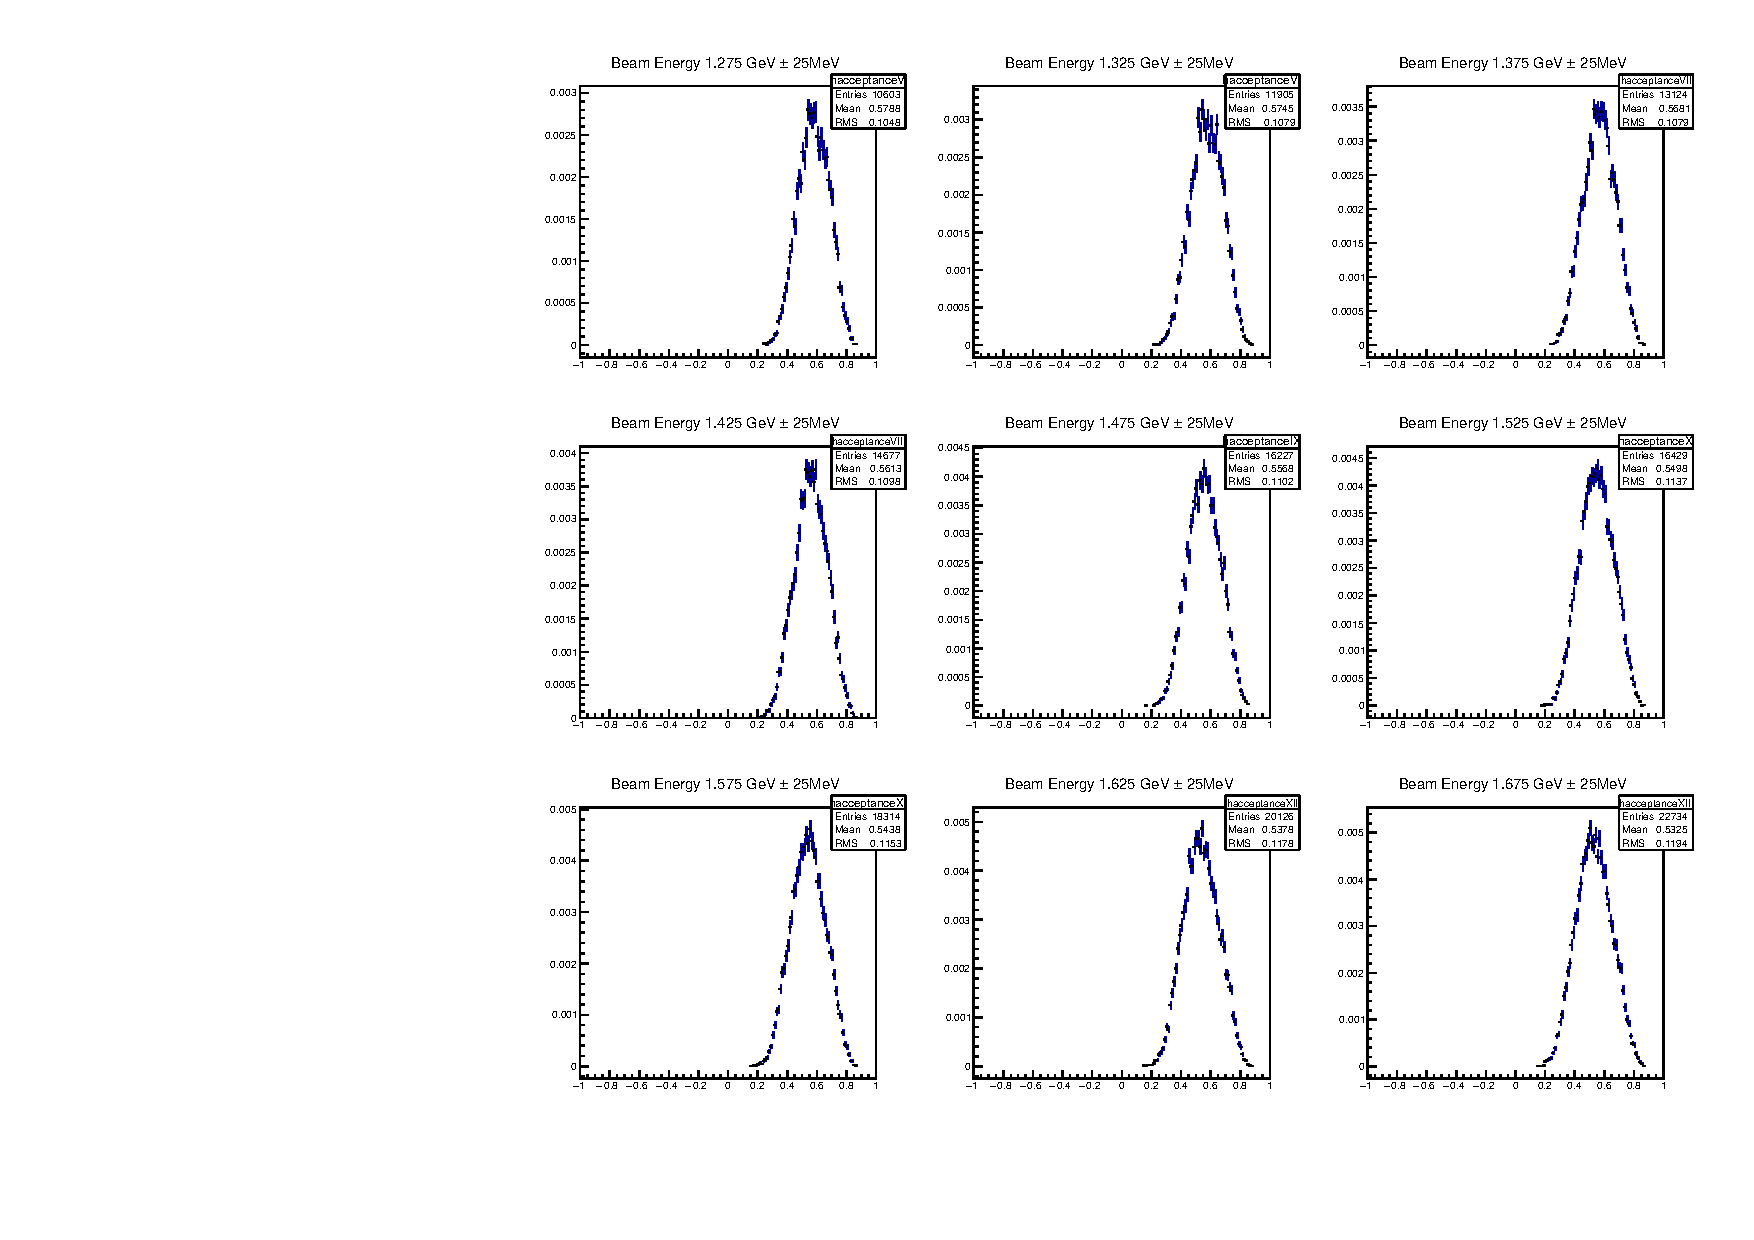
\includepdf[pages=-]{AcceptanceAll.pdf}
%/Volumes/Mac_Storage/Work_Data/CONVERSION_SIM/PHASESPACE/ACCEPTANCE/PLOTS/Acceptance_All.pdf
\end{document}